\begin{dang}{Cực trị khoảng cách}
\end{dang}
\subsubsection{Ví dụ mẫu}
%VD1
\begin{vd}[VDT]%[Nguyễn Văn Hiệp]%[1K7GP-7]
	Cho hình chóp đều $S.ABC$ có cạnh đáy bằng $a$, cạnh bên bằng $\dfrac {2a\sqrt {3}}{3}$ và $O$ là tâm của đáy. Mặt phẳng $(P)$ thay đổi chứa $SO$ và cắt các đoạn thẳng $AB$, $AC$ lần lượt tại các điểm $M, N$
	($M,N$ khác $A$). Khi góc tạo bởi đường thẳng $SA$ và mặt phẳng $(P)$ có số đo lớn nhất, hãy tính $AM^2+AN^2$.
	\dapso{$AM^2+AN^2=\dfrac {8a^2}{9}$.}
	\loigiai{
		\begin{center}
			\begin{tikzpicture}
				\def\a{5}
				\def\h{5}
				\path 	(0:0) coordinate (B)
				++(0:\a) coordinate (C)
				++(-150:4*\a/5) coordinate (A)
				($(B)!0.5!(C)$) coordinate (I)
				($(A)!0.6!(B)$) coordinate (M)
				($(A)!2/3!(I)$) coordinate (O)
				($(O)+(90:\h)$) coordinate (S)
				(intersection of M--O and A--C) coordinate (N)
				($(M)!0.3!(O)$) coordinate (H)
				;
				\draw[thick] (B)--(A)--(C)
				(A)--(S)	(B)--(S)	(C)--(S);
				\draw[dashed,thick] (A)--(I) (S)--(O) (B)--(C) (M)--(O)--(N) (A)--(H)--(S);
				\foreach \x / \goc in {A/-90,B/180,C/0,O/-45,I/45,S/90,M/180,N/-30,H/135}
				\fill (\x) circle (1.5pt)
				($(\x)+(\goc:3mm)$) node {$\x$};
				\path pic[draw,angle radius=5pt]{right angle= O--H--A};
			\end{tikzpicture}
		\end{center}
		Gọi $H$ là hình chiếu của $A$ trên $MN$, ta có $AH\perp MN$, $AH\perp SO\Rightarrow AH\perp ( SMN )$.\\
		$\Rightarrow H$ là hình chiếu của $A$ trên mặt phẳng $( SMN )$.\\
		$\Rightarrow $ Góc giữa đường thẳng $SA$ và mặt phẳng $( SMN )$ là góc $\widehat{HSA}$.\\
		Do góc $0^\circ<\widehat{HSA}<90^\circ$ nên $\widehat{HSA}$ lớn nhất khi $\sin \widehat{HSA}$ lớn nhất.\\
		Ta có $\sin \widehat{HSA}=\dfrac {AH}{SA}\le \dfrac {OA}{SA}\le \dfrac {\dfrac {a\sqrt {3}}{3}}{\dfrac {2a\sqrt {3}}{3}}\le \dfrac {1}{2}$.\\
		Vậy $\sin \widehat{HSA}$ đạt giá trị lớn nhất bằng $\dfrac {1}{2}$ khi $H\equiv O$.\\
		Hay góc giữa đường thẳng $SA$ và mặt phẳng $(P)$ đạt giá trị lớn nhất khi $MN\perp AO$.\\
		Khi đó đường thẳng $MN$ đi qua $O$ và song song với $BC$ $\Rightarrow AM=AN=\dfrac {2}{3}a\Rightarrow AM^2+AN^2=\dfrac {8a^2}{9}$.
	}
\end{vd}
%VD2
\begin{vd}[VDC]%[DCHT Toán 11 - KNTT -Nguyễn Văn Hiệp]%[1K7GP-7]
	Cho hình thoi $ABCD$ có $\widehat{BAD}=60^\circ$, $AB=2a$. Gọi $H$ là trung điểm $AB$, trên đường thẳng $ d$ vuông góc với mặt phẳng $( ABCD )$ tại $H$ lấy điểm $S$ thay đổi khác $H$. Biết rằng góc giữa $SC$ và $( SAD )$ có số đo lớn nhất khi $SH=a \sqrt [4]{\dfrac {m}{n}}$( với $ m,n$ là các số tự nhiên và $\dfrac {m}{n}$ là phân số tối giản). Khi đó tổng $ m+n$ bằng?
	\dapso{$m+n=25$.}
	\loigiai{
		\begin{center}
			\begin{tikzpicture}
				\def\a{4}
				\path 	(0:0) coordinate (B)
				++(0:\a) coordinate (C)
				++(-120:\a) coordinate (D)
				($(B)+(D)-(C)$) coordinate (A)
				($(A)!0.5!(B)$) coordinate (H)
				($(H)+(90:\a*1.2)$) coordinate (S)
				($(A)!0.4!(D)$) coordinate (E)
				(intersection of A--C and B--D) coordinate (O);%giao điểm O
				\draw[dashed,thick] 	(A)--(B)--(C)	(B)--(S) (S)--(H)--(C) (H)--(E);
				\draw[thick] 			(A)-- (D)--(C)
				(A)--(S)	(C)--(S)	(D)--(S)--(E);
				\foreach \x/\g in {A/-135,B/180,C/0,D/-45,S/90,H/180,E/-90}
				\fill[black] 	(\x) circle (1pt)
				($(\g:3mm)+(\x)$) node {$\x$};
				\foreach \x/\y/\z in {C/H/S,D/E/H}{
					\path pic[draw,angle radius=5pt]{right angle= \x--\y--\z};
				}
			\end{tikzpicture}
			\hspace*{1cm}
			\begin{tikzpicture}[declare function={r=5;}]
				\path 	(0:0) coordinate (B)
				++(0:r) coordinate (I)
				++(-120:r*0.5) coordinate (D)
				($(B)+(D)-(I)$) coordinate (A)
				($(A)!0.3!(I)$) coordinate (S)
				($(S)+(20:0.5*r)$) coordinate (M)
				($(M)+(90:0.5*r)$) coordinate (C)
				(intersection of S--C and B--I) coordinate (E)
				(intersection of M--C and B--I) coordinate (F)
				;
				\draw[dashed] (E)--(F);
				\draw[thick] (B)--(E) (F)--(I)--(D)--(A)--(B)
				(S)--(M)--(C)--cycle
				;
				\path pic[draw,angle radius=34pt]{angle= D--A--B};
				\node[shift={(20:0.7)}] at (A) {$SAD$};
				\foreach \t/\g in {S/-90,M/0,C/90}{
					\fill (\t) circle (1pt) node[shift={(\g:7pt)},font=\scriptsize]{$ \t $};
				}
				\path pic[draw,angle radius=5pt]{right angle= C--M--S};
				\path pic[draw,angle radius=7pt]{angle= M--S--C};
			\end{tikzpicture}
		\end{center}
		Gọi $M$ là hình chiếu của $C$ lên $(SAD)$ và $\varphi $ là góc giữa $SC$ và$(SAD)$.\\
		Ta có $\sin \varphi =\dfrac {CM}{SC}=\dfrac {\mathrm{d}(C,(SAD))}{SC}$.\\
		Vì $BC \parallel(SAD)\Rightarrow \mathrm{d}(C,(SAD))=\mathrm{d}(B,(SAD) )=2\mathrm{d}(H,(SAD))$.\\
		Gọi $E$ là hình chiếu của $H$ trên $AD$và $F$ là hình chiếu của $H$ trên $SE$,
		ta có $\mathrm{d}(H,(SAD) )=HF$.\\
		Khi đó $\sin \varphi =\dfrac {2HF}{SC}$.\\
		Đặt $SH=x~(x>0),$ vì tam giác $SHC$ vuông tại $H$ nên $$SC=\sqrt {SH^2+CH^2}=\sqrt {SH^2+BC^2+BH^2-2BC\cdot BH\cdot \cos\widehat{CBH}}=\sqrt {x^2+7a^2}.$$
		Tam giác vuông $EHA$ có $\sin \widehat{HAE}=\dfrac {HE}{AH}\Rightarrow HE=\dfrac {a\sqrt {3}}{2}$.\\
		Do $HF$ là đường cao của tam giác vuông $HSE$ nên $\dfrac {1}{HF^2}=\dfrac {1}{HE^2}+\dfrac {1}{HS^2}=\dfrac {4}{3a^2}+\dfrac {1}{x^2}\Rightarrow HF=\dfrac {ax\sqrt {3}}{\sqrt {3a^2+4x^2}}$.\\
		Khi đó
		$\sin \varphi =\dfrac {2HF}{SC}=\dfrac {2\sqrt {3}ax}{\sqrt {(4x^2+3a^2)(x^2+7a^2)}}=\dfrac {2\sqrt {3}ax}{\sqrt {(4x^4+21a^4)+31a^2x^2}}$.\\
		$\Rightarrow \sin \varphi \le \dfrac {2\sqrt {3}ax}{\sqrt {4\sqrt {21}\cdot a^2x^2+31\cdot a^2\cdot x^2}}\Rightarrow \sin \varphi \le \sqrt {\dfrac {12}{4\sqrt {21}+31}} $\\
		Dấu đẳng thức xảy ra khi $ x=\sqrt [4]{\dfrac {21}{4}}a$.\\
		Vậy $\varphi $ lớn nhất khi và chỉ khi $\sin \varphi $ lớn nhất khi và chỉ khi $SH=\sqrt [4]{\dfrac {21}{4}}a\Rightarrow m=21,n=4$.\\
		Khi đó $ m+n=21+4=25$.
	}
\end{vd}
%VD3
\begin{vd}[VDC]%[DCHT Toán 11 - KNTT -Nguyễn Văn Hiệp]%[1K7GP-7]
	Cho hình lăng trụ tam giác đều $ABC.A'B'C'$ có tất cả các cạnh bằng $1$. Gọi $M$ là điểm nằm trên cạnh $AA'$ sao cho mặt phẳng $(C'MB)$ tạo với mặt phẳng $(ABC)$ một góc nhỏ nhất. Tính diện tích tam giác $C'MB$.
	\dapso{$S_{C'MB}=\dfrac {\sqrt {6}}{4}$.}
	\loigiai{
		\begin{center}
			\begin{tikzpicture}
				\def\a{4}
				\def\h{4.5}
				\path 	(0:0) coordinate (A)
				++(0:\a) coordinate (C)
				++(-150:3*\a/4) coordinate (B)
				($(A)+(90:\h)$) coordinate (A')
				($(B)+(90:\h)$) coordinate (B')
				($(C)+(90:\h)$) coordinate (C')
				($(A)!0.3!(A')$) coordinate (M)
				($(A)!0.5!(C)$) coordinate (I)
				(intersection of C'--M and C--A) coordinate (E)
				($(B)!0.3!(E)$) coordinate (H)
				(intersection of C'--H and M--B) coordinate (K)
				;
				\draw[dashed,thick] 	(A)--(C) (K)--(C')--(M)--(A) (B)--(I) (B)--(A)--(E) ;
				\draw[thick]	(C)--(C') 	(B)--(B')	(M)--(A') (B)--(C) (A')--(B')--(C')--cycle (B)--(H)--(E)--(M) (A')--(B)--(M) (K)--(H);
				\foreach \x/\g in {A/135,B/-90,C/0,A'/180,B'/90,C'/0,E/180,H/-150,I/90,M/150}
				\fill[black] 	(\x) circle (1pt)
				($(\g:4mm)+(\x)$) node {$\x$};	
				\foreach \x/\y/\z in {B/I/C,B/H/C'}{
					\path pic[draw,angle radius=5pt]{right angle= \x--\y--\z};
				}
			\end{tikzpicture}
		\end{center}
		
		Đặt $AM=x$, $0\le x\le 1$.\\
		Gọi $E$ là giao điểm của $C'M$ và $AC$. Ta có $(C'MB)\cap (ABC)=EB$.\\
		Kẻ $C'H\perp EB$ tại $H$ thì $C'H=\mathrm{d}(C',EB)$.\\
		Suy ra $\sin ((C'MB),(ABC))=\dfrac {\mathrm{d}(C',(ABC))}{\mathrm{d}(C',EB)}=\dfrac {CC'}{C'H}$.\\
		Do đó, góc giữa mặt phẳng $(C'MB)$ và mặt phẳng $(ABC)$ nhỏ nhất khi $C'H$ lớn nhất.\\
		Ta có: $AM\parallel CC'\Rightarrow \dfrac {EA}{EC}=\dfrac {AM}{CC'}=x\Rightarrow EA=xEC=x(1+EA)$.\\
		Suy ra $EA=\dfrac {x}{1-x}$ và $EC=EA+AC=\dfrac {1}{1-x}$. (với $ x\ne 1$ ).\\
		Xét tam giác $EAB$ có
		\begin{eqnarray*}
			EB&=&\sqrt {EA^2+AB^2-2EA\cdot AB\cdot \cos \widehat{EAB}}\\ 
			&=&\sqrt {\left( \dfrac {x}{1-x} \right)^2+1^2-2\dfrac {x}{1-x}\cdot 1\cdot \cos 120^\circ }=\dfrac {\sqrt {x^2-x+1}}{1-x}. 
		\end{eqnarray*}
		Gọi $I$ là trung điểm của $AC$. Khi đó
		$$S_{EBC}=\dfrac {1}{2}CH\cdot EB=\dfrac {1}{2}BI\cdot EC\Rightarrow CH=\dfrac {BI\cdot EC}{EB}=\dfrac {\dfrac {\sqrt {3}}{2}\cdot \dfrac {1}{1-x}}{\dfrac {\sqrt {x^2-x+1}}{1-x}}=\dfrac {\sqrt {3}}{2\sqrt {x^2-x+1}}.$$
		Do đó $C'H=\sqrt {CH^2+CC'^2}=\sqrt {\dfrac {3}{4(x^2-x+1)}+1}=\sqrt {\dfrac {3}{4\left( x-\dfrac {1}{2} \right)^2+3}+1}\le \sqrt {2}$.\\
		Từ đây suy ra $C'H_{\max}=\sqrt {2}$ xảy ra khi $x=\dfrac {1}{2}$ hay $M$ là trung điểm của $AA'$.\\
		Khi đó, $\sin \left((C'MB),(ABC)\right)=\dfrac {CC'}{C'H}=\dfrac {1}{\sqrt {2}}\Rightarrow \left((C'MB),(ABC)\right)=45^\circ$.\\
		Vì $\triangle ABC$ là hình chiếu vuông góc của $\Delta C'MB$ lên $ mp(ABC)$ nên
		$$S_{ABC}=S_{C'MB}\cdot \cos \left(({C}'MB),(ABC)\right)\Rightarrow S_{C'MB}=\dfrac {S_{ABC}}{\cos \left((C'MB),(ABC)\right)}=\dfrac {\dfrac{\sqrt {3}}{4}}{\dfrac{\sqrt {2}}{2}}=\dfrac {\sqrt {6}}{4}.$$
		Khi $ x=1$ ta có $M$ trùng với $A'$ và mặt phẳng $(C'MB)$ trùng với $(C'A'B)$ tạo với mặt phẳng $(ABC)$ một góc bằng $\alpha $ với $\tan \alpha =\dfrac {2\sqrt {3}}{3}>1$.\\
		Vậy $S_{C'MB}=\dfrac {\sqrt {6}}{4}$.
	}
\end{vd}
%VD4
\begin{vd}[VDT]%[DCHT Toán 11 - KNTT -Nguyễn Văn Hiệp]%[1K7GP-7]
	Cho hình lập phương $ABCD.A'B'C'D'$ cạnh bằng $a$. Trong các mặt phẳng chứa đường thẳng $CD'$, gọi $(\alpha)$ là mặt phẳng tạo với $(BDD'B')$ một góc nhỏ nhất. Tính $ d(A,(\alpha))$
	\dapso{$\dfrac {a\sqrt {6}}{2}$.}
	\loigiai{
		\begin{itemize}
			\item Gọi $\Delta =(\alpha)\cap (BDD'B')$.
			\item Ta có $CO\perp (BDD'B')$. Kẻ $OH\perp \Delta \Rightarrow CH\perp \Delta $ $\Rightarrow \varphi =\widehat{((\alpha),(BDD'B'))}=\widehat{( OH,CH )}=\widehat{OHC}$.
			\item $\sin \varphi =\dfrac {OC}{CH}\ge \dfrac {OC}{CD'}=\sin \widehat{OD'C}\Rightarrow \min \varphi =\widehat{OD'C}$, đạt được khi $\Delta \perp OD'$.\\
			Gọi $E=\Delta \cap BD\Rightarrow (\alpha)\equiv (ED'C)$.\\
			$OD\cdot OE=OD'^2\Rightarrow \dfrac {a\sqrt {2}}{2}\cdot OE=\left( \dfrac {a\sqrt {6}}{2} \right)^2\Rightarrow OE=\dfrac {3a\sqrt {2}}{2}\Rightarrow DE=a\sqrt {2}$.\\
			Suy ra $E$ đối xứng với $B$ qua $D$.
			\item Có $\mathrm{d}(A,(\alpha) )=3\mathrm{d}(D,(\alpha))$.
			\item Kẻ $DK\perp CE$, $(K\in CE)$; kẻ $DF\perp D'K,~(F\in D'K )\Rightarrow DF\perp (\alpha)\Rightarrow \mathrm{d}(D,(\alpha))=DF$.\\
			Ta có $DK=\dfrac {a}{\sqrt {5}}$; $DD'=a\Rightarrow DF=\dfrac {a\sqrt {6}}{6}\Rightarrow \mathrm{d}(A,(\alpha))=3\cdot DF=\dfrac {a\sqrt {6}}{2}$.
		\end{itemize}
		
	}
\end{vd}
%VD5
\begin{vd}[VDT]%[DCHT Toán 11 - KNTT -Nguyễn Văn Hiệp]%[1K7GP-7]
	Cho tứ diện đều có cạnh bằng $3$. $M$ là một điểm thuộc miền trong của khối tứ diện tương ứng. Tính giá trị lớn nhất của tích các khoảng cách
	từ điểm $M$ đến bốn mặt của tứ diện đã cho. 
	\dapso{$\dfrac{9}{64}$.}
	\loigiai{Gọi$r_1$, $r_2$, $r_3$, $r_4$ là khoảng cánh từ điểm $M$ đến bốn mặt của tứ diện.\\
		Gọi $S$ là diện tích một mặt của tứ diện $\Rightarrow S=\dfrac{9\sqrt{3}}{4}$.\\
		Đường cao của tứ diện là $h=\sqrt{3^2-\left(\sqrt{3}\right)^2}=\sqrt{6}$.\\
		Thể tích của tứ diện là $V=\dfrac{1}{3} S\cdot h=\dfrac{1}{3}\cdot \dfrac{9\sqrt{3}}{4}\cdot \sqrt{6}=\dfrac{9\sqrt{2}}{4}$.\\
		Mặt khác, ta có $V=\dfrac{1}{3}\cdot S\cdot \left(r_1+r_2+r_3+r_4\right)=\dfrac{9\sqrt{2}}{4}\Rightarrow r_1+r_2+r_3+r_4=3\dfrac{9\sqrt{2}}{4}\dfrac {4}{9\sqrt{3}}=\sqrt{6}$.\\
		Lại có $\sqrt{6}=r_1+r_2+r_3+r_4\ge 4\sqrt[4]{r_1 \cdot r_2\cdot r_3 \cdot r_4}\Leftrightarrow r_1\cdot r_2 \cdot r_3 \cdot r_4 \le \dfrac{9}{64}$.
	}
\end{vd}

\subsubsection{Bài tập trắc nghiệm}
\Opensolutionfile{ans}[ans/ans-1K7-26-Dang8]%

\begin{ex}%[DCHT Toán 11 - KNTT -Nguyễn Văn Hiệp]%[1K7GP-7]
	Cho hình thang vuông $ABCD$ vuông ở $A$ và $D$, $AD= 2a$. Trên đường thẳng vuông góc tại $D$ với $ABCD$ lấy điểm $S$ với $SD=a\sqrt{2}$. Biết điểm $M$ di động trên đường thẳng $CD$, tìm giá trị nhỏ nhất khoảng cách từ điểm $M$ đến đường thẳng $SA$. 
	\choice
	{\True $\dfrac{2a}{\sqrt{3}}$}
	{$\dfrac{a}{\sqrt{2}}$}
	{$a\sqrt{2}$}
	{$\dfrac{a\sqrt{3}}{3}$}
	\loigiai{\immini{Dễ thấy khoảng cách này bằng khoảng cách từ điểm $D$ đến đường thẳng $SA$.\\
			Trong tam giác vuông $SAD$ ta có
			$$\dfrac{1}{DH^2}=\dfrac{1}{SA^2}+\dfrac{1}{AD^2}\Rightarrow DH=\dfrac{SA\cdot AD}{SA^2+AD^2}=\dfrac{2a}{\sqrt{3}}.$$}{
			\begin{tikzpicture}
				\def\a{5}
				\def\h{4}
				\path 	(0:0) coordinate (D)
				++(0:\a) coordinate (C)
				($(D)+(-130:\a/2)$) coordinate (A)
				($(A)+(C)-(D)$) coordinate (Bt)
				($(A)!1/2!(Bt)$) coordinate (B)
				($(D)+(90:\h)$) coordinate (S)
				($(A)!(D)!(S)$) coordinate (H)
				;
				\draw[dashed,thick] 	(A)--(D)--(C)	(D)--(S) (D)--(H);
				\draw[thick] 			(A)--(B)--(C)
				(A)--(S)	(B)--(S)	(C)--(S);
				\foreach \x/\g in {A/-135,B/-45,C/0,D/-60,S/90,H/160}
				\fill[black] 	(\x) circle (1pt)
				($(\g:3mm)+(\x)$) node {$\x$};	
				\foreach \x/\y/\z in {C/D/S,D/H/S}{
					\path pic[draw,angle radius=5pt]{right angle= \x--\y--\z};
				}
		\end{tikzpicture}}
	}
\end{ex}
%Cau2
\begin{ex}%[DCHT Toán 11 - KNTT -Nguyễn Văn Hiệp]%[1K7GP-7]
	Cho tứ diện $ABCD$ có các cạnh vuông góc với nhau đôi một và $AD=2AC=3AB=a$. Gọi $\Delta$ là đường thẳng chứa trong mặt $(BCD)$ sao cho khoảng cách từ điểm $A$ đến $\Delta$ là nhỏ nhất và khoảng cách lớn nhất giữa hai đường thẳng $\Delta$ và $AD$ là $d$. Khẳng định nào sau đây là đúng?
	\choice
	{$\dfrac{a\sqrt{14}}{14}$}
	{$3a<d<4a$}
	{\True $\dfrac{3a}{14}<d<\dfrac{4a}{7}$}
	{$d>4a$}
	\loigiai
	{\immini{Gọi $H$ là hình chiếu vuông góc của $A$ lên $(BCD)$. Khi đó ta có $H$ là trực tâm của tam giác $BCD$.\\
			Với mọi đường thẳng $\Delta$ nằm trong $(BCD)$ thì $\mathrm{d}(A,\Delta)\ge AH$. Do đó đường thẳng $\Delta$ thỏa mãn phải đi qua điểm $H$.\\
			Kẻ $HK \perp AD$ $(K \in AD)$ khi đó $H,K$ là hai điểm cố định lần lượt nằm trên $\Delta$ và $AD$.\\
			Hiển nhiên, khoảng cách giữa $\Delta$ và $AD$ là độ dài đoạn vuông góc chung của chúng nên $\mathrm{d}(\Delta; AD)\le HK$.\\ Dấu bằng xảy ra khi $HK\perp \Delta$.\\
			Ta có $$\dfrac {1}{AH^2}=\dfrac {1}{AB^2}+\dfrac {1}{AC^2}+\dfrac {1}{AD^2}=\dfrac {1}{\left(\dfrac {a}{3}\right)^2}+\dfrac {1}{\left(\dfrac {a}{2}\right)^2}+\dfrac {1}{a^2}=\dfrac {14}{a^2}\Rightarrow AH= \dfrac {a}{\sqrt{14}}.$$
			Ta có $$\cos \widehat{HAK}=\dfrac{AH}{AD}=\dfrac{1}{\sqrt{14}}\Rightarrow \sin \widehat{HAK}=\dfrac{\sqrt{13}}{\sqrt{14}}\Rightarrow HK=HA\sin \widehat{HAK}=\dfrac{a\sqrt{13}}{14}\Rightarrow \dfrac{3a}{14}<d<\dfrac{4a}{7}.$$}
		{
			\begin{tikzpicture}
				\def\a{5}
				\def\h{4}
				\path 	(0:0) coordinate (B)
				++(0:\a) coordinate (D)
				++(-150:4*\a/5) coordinate (C)
				($(B)!0.5!(D)$) coordinate (M)
				($(C)!2/3!(M)$) coordinate (H)
				($(H)+(90:\h)$) coordinate (A)
				($(A)!(H)!(D)$) coordinate (K)
				;
				\draw[thick] (B)--(C)--(D)
				(B)--(A)	(C)--(A)	(D)--(A) ;
				\draw[dashed,thick] (B)--(D) (A)--(H) 	(C)--(M) (H)--(K);
				\foreach \x / \goc in {B/180,D/0,C/-135,H/-60,A/90,K/45}
				\fill (\x) circle (1.5pt)
				($(\x)+(\goc:3mm)$) node {$\x$};
				\foreach \x/\y/\z in {B/A/C,C/A/D,A/H/B,A/K/H}{
					\path pic[draw,angle radius=5pt]{right angle= \x--\y--\z};
				}
		\end{tikzpicture}}
	}
\end{ex}
%Cau3
\begin{ex}%[DCHT Toán 11 - KNTT -Nguyễn Văn Hiệp]%[1K7GP-7]
	Cho hình chóp $S.ABC$ có $AB=BC=CA=2a$, $SA=SB=SC=3a$, $J$ là điểm bất kì trong không gian. Gọi $h$ là tổng khoảng cách từ $J$ đến tất cả các đường thẳng $AB$, $BC$, $CA$, $SA$, $SB$, $SC$. Giá trị nhỏ nhất của $h$ bằng
	\choice
	{$a\sqrt{21}$}
	{\True $a\sqrt{23}$}
	{$\dfrac {a\sqrt{23}}{2}$}
	{$\dfrac{a\sqrt{21}}{2}$}
	\loigiai{
		\begin{center}
			\begin{tikzpicture}[declare function={r=4;}]
				\path (160:{r} and {r*0.35}) coordinate(A)
				(260:{r} and {r*0.5}) coordinate (C)
				(20:{r} and {r*0.35})coordinate (B)
				(90:{r*1.25}) coordinate (S)
				($(B)!.5!(C)$) coordinate (M)
				($(A)!.5!(C)$) coordinate (N)
				($(A)!.5!(B)$) coordinate (P)
				($(S)!.5!(A)$) coordinate (A')
				($(S)!.5!(B)$) coordinate (B')
				(intersection of A'--M and N--B') coordinate (I)
				(intersection of S--I and A--M) coordinate (O)
				(intersection of P--I and S--C) coordinate (C')
				;
				\draw[thick,dash pattern=on 2pt off 2 pt] (A)--(B) (A')--(M) (N)--(B') (S)--(O) (P)--(C') (A)--(O)--(M);
				\draw[thick] (A)--(C)--(B)--(S)--cycle (S)--(C) (S)--(M);
				\foreach \t/\g in {A/180,B/0,C/-90,S/90, M/-90,N/-135,P/-90,A'/140,B'/45,C'/130,I/0,O/-90}{
					\fill (\t) circle (1pt) node[shift={(\g:7pt)},font=\scriptsize]{$ \t $};
				}
				\foreach \x/\y/\z in {M/O/S,S/A'/M,S/B'/N}{
					\path pic[draw,angle radius=5pt]{right angle= \x--\y--\z};
				}
			\end{tikzpicture}	
		\end{center}	
		Theo đề ta có hình chóp $S.ABC$ là hình chóp đều.\\
		Gọi $O$ là tâm của đáy. Khi đó $SO$ là chiều cao của hình chóp.
		Gọi $M,~N,~P$ lần lượt là trung điểm của $BC$, $AC$, $AB$; gọi $A',~B',~C'$ lần lượt là hình chiếu của $M,~N,~P$ lên các cạnh $SA$, $SB$, $SC$.\\
		Ta có $\heva{&BC \perp AM\\& BC \perp SM}\Rightarrow BC \perp (SAM)\Rightarrow BC \perp MA'$.\\
		Vậy $MA'$ là đường vuông góc chung của các cạnh $SA$, $BC$.\\
		Chứng minh tương tự ta có $NB'$ là đường vuông góc chung của $SB$ và $AC$; $PC'$ là đường vuông góc chung của $AB$, $SC$.\\
		Do các $\triangle SMA$, $\triangle SNB$, $\triangle SPC$ bằng nhau và $MA'$, $NB'$, $PC'$ là những đường cao tương ứng nên ta có $MA'=NB'=PC$ đồng thời $SA'=SB'=SC'$.\\
		Vì $\dfrac {SA'}{SA}=\dfrac {SC'}{SC}$ nên ta có $A'C'\parallel AC \Rightarrow PM \parallel A'C' \Rightarrow$ Bốn điểm $M,~P,~A',~C'$ đồng phẳng.\\
		Chứng minh tương tự ta có $M,~N,~A',~B'$ đồng phẳng và $P,~N,~B',~C'$ đồng phẳng.\\
		Do các mặt $(MPA'C')$, $(MNA'B')$, $(PNB'C')$ lần lượt cắt nhau theo ba giao tuyến $MA'$, $NB'$, $PC'$ nên chúng đồng quy tại $I$ (Với $I\in SO$).\\
		Gọi $J$ là điểm bất kỳ trong không gian.\\
		Ta có $$\heva{&\mathrm{d}(J,SA)+\mathrm{d}(J,BC) \ge MA'\\&\mathrm{d}(J,SB)+\mathrm{d}(J,AC) \ge NB'\\& \mathrm{d}(J,SC)+\mathrm{d}(J,AB) \ge PC'}\Rightarrow h \ge MA'+NB'+PC'=3MA'.$$
		Vậy $h_{\text{min}}=3MA'$ khi $J\equiv I$.\\
		Trong tam giác $SOA$ vuông tại $O$ có $\sin \widehat{ASO}=\cos \widehat{SAO}= \dfrac{AO}{SA}=\dfrac{\dfrac{2a\sqrt{3}}{3}}{3a}=\dfrac{2\sqrt{3}}{9}\Rightarrow \sin \widehat{SAO}=\dfrac{\sqrt{69}}{9}$.\\
		Trong tam giác $MAA'$ vuông ở $A'$ có $\sin \widehat{MAA'}=\dfrac{MA'}{MA}\Rightarrow MA'=a\sqrt{3}\cdot \dfrac{\sqrt{69}}{9}=\dfrac{a\sqrt{23}}{3}$.\\
		Vậy $h_{\text{min}}=3MA'=a\sqrt{23}$.
	}
\end{ex}
%Cau4
\begin{ex}%[DCHT Toán 11 - KNTT -Nguyễn Văn Hiệp]%[1K7GP-7]
	Cho hình lập phương $ABCD.A'B'C'D'$ có cạnh bằng $a$, $M$ là điểm thay đổi trong không gian. Giá trị nhỏ nhất của biểu thức $T=MA^2+MB^2+MC^2+MD^2+MA'^2+MB'^2+MC'^2+MD'^2$ bằng
	\choice
	{$6a^2$}
	{\True $8a^2$}
	{$3a^2$}
	{$4a^2$}
	\loigiai
	{\begin{center}
			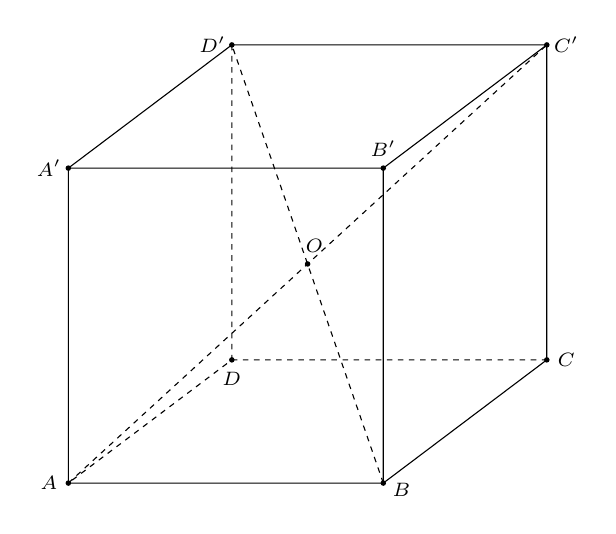
\begin{tikzpicture}[declare function={r=4;}]
				\path (0:0) coordinate (A)
				(0:r) coordinate (B)
				++(37:{0.65*r}) coordinate (C)
				++(180:r) coordinate (D)
				\foreach \x in {A,B,C,D}{(\x)++(90:r) coordinate (\x')}
				(intersection of A--C' and B--D') coordinate (O)
				;
				\draw[dash pattern=on 2pt off 2 pt] (D')--(D)--(A) (D)--(C) (A)--(C') (B)--(D');
				\draw (A)--(B)--(C) (A)--(A') (B)--(B') (C)--(C') (A')--(B')--(C')--(D')--cycle;
				\foreach \t/\g in {A/180,B/-20,C/0,D/-90,A'/180,B'/90,C'/0,D'/180,O/70}{
					\fill (\t) circle (1pt) node[shift={(\g:7pt)},font=\scriptsize]{$ \t $};
				}
			\end{tikzpicture}
		\end{center}
		Gọi $O$ là tâm của hình lập phương $\Rightarrow OA=OB=OC=OD=OA'=OB'=OC'=OD'=\dfrac{a\sqrt{3}}{2}$.\\
		Gọi $I$ là điểm thỏa mãn $\vec{IA}+\vec{IB}+\vec{IC}+\vec{ID}+\vec{IA'}+\vec{IB'}+\vec{IC'}+\vec{ID'}=\vec{0}$.\\
		$\Leftrightarrow \left(\vec{IA}+\vec{IC'}\right)+\left(\vec{IB}+\vec{ID'}\right)+\left(\vec{IC}+\vec{IA'}\right)+\left(\vec{ID}+\vec{IB'}\right)=\vec{0}$\\
		$\Leftrightarrow 2\vec{IO}+2\vec{IO}+2\vec{IO}+2\vec{IO}=\vec{0}\Leftrightarrow \vec{IO}=\vec{0}\Leftrightarrow I\equiv O$.\\
		Ta có 
		\allowdisplaybreaks
		\begin{eqnarray*}
			T&=&MA^2+MB^2+MC^2+MD^2+MA'^2+MB'^2+MC'^2+MD'^2\\
			&=&\left(\vec{MI}+\vec{IA}\right)^2+ \left(\vec{MI}+\vec{IB}\right)^2+ \left(\vec{MI}+\vec{IC}\right)^2+ \left(\vec{MI}+\vec{ID}\right)^2+ \left(\vec{MI}+\vec{IA'}\right)^2+ \left(\vec{MI}+\vec{IB'}\right)^2\\ &+&\left(\vec{MI}+\vec{IC'}\right)^2+ \left(\vec{MI}+\vec{ID'}\right)^2\\
			&=&8MI^2+ 2\vec{MI}\left(\vec{IA}+\vec{IB}+\vec{IC}+\vec{ID}\vec{IA'}+\vec{IB'}+\vec{IC'}+\vec{ID'}\right) + IA^2+IB^2+IC^2+ID^2+IA'^2\\
			&+&IB'^2+IC'^2+ID'^2\\
			&=&8MI^2+ OA^2+OB^2+OC^2+OD^2+OA'^2+OB'^2+OC'^2+OD'^2\\
			&=&8MI^2+6a^2 \ge 6a^2.
		\end{eqnarray*}
		$\Rightarrow T_{\text{min}}=6a^2$.\\
		Dấu bằng xảy ra khi $M\equiv I\equiv O$.
	}
\end{ex}

%Cau 5
\begin{ex}%[DCHT Toán 11 - KNTT -Nguyễn Văn Hiệp]%[1K7GP-7]
	Cho hình chóp $S.ABC$ với $SA=3$, $SB=4$, $SC=5$. Một mặt phẳng $\alpha$ thay đổi luôn đi qua trọng tâm của $S.ABC$ cắt các cạnh $SA$, $SB$, $SC$ lần lượt tại các điểm $A_1$, $B_1$, $C_1$. Tìm giá trị nhỏ nhất của biểu thức $P=\dfrac{1}{SA_1^2} + \dfrac{1}{SB_1^2} +\dfrac{1}{SC_1^2}$
	\choice
	{$\dfrac{7}{16}$}
	{$\dfrac{5}{16}$}
	{$\dfrac{7}{25}$}
	{\True $\dfrac{8}{25}$}
	\loigiai{
		Gọi $G$ là trọng tâm của $S.ABC$ khi đó $\vec{GA}+\vec{GB}+\vec{GC}+\vec{GS}=\vec{0}$.\\
		Từ đó $\vec{SG}=\dfrac{1}{4}\left(\vec{SA}+\vec{SB}+\vec{SC}\right)\quad (1)$.\\
		Do $A_1$, $B_1$, $C_1$ thuộc các tia $SA$, $SB$, $SC$ nên $\vec{SA}$, $\vec{SA_1}$ cùng hướng; $\vec{SB}$, $\vec{SB_1}$ cùng hướng; $\vec{SC}$, $\vec{SC_1}$ cùng hướng từ đó
		$\dfrac{\vec{SA}}{SA}=\dfrac{\vec{SA_1}}{SA_1}$, $\dfrac{\vec{SB}}{SB}=\dfrac{\vec{SB_1}}{SB_1}$, $\dfrac{\vec{SC}}{SC}=\dfrac{\vec{SC_1}}{SC_1}$.\\
		Vậy $(1)$ tương đương với 
		$$\vec{SG}=\dfrac{1}{4}\left(\dfrac{SA}{SA_1}\vec{SA_1}+ \dfrac{SB}{SB_1}\vec{SB_1}+ \dfrac{SC}{SC_1}\vec{SC_1}\right)\quad (2)$$
		Do $G$, $A_1$, $B_1$, $C_1$ thuộc một mặt phẳng nên từ $(2)$ ta có $\dfrac{1}{4}\left(\dfrac{SA}{SA_1}+\dfrac{SB}{SB_1}+ \dfrac{SC}{SC_1}\right)=1$.\\
		Hay $\dfrac{3}{x}+\dfrac{4}{y}+\dfrac{5}{z}=4$ trong đó $x=SA_1$, $y=SB_1$, $z=SC_1$.\\
		Bài toán quy về tìm giá trị nhỏ nhất của $P=\dfrac{1}{x^2}+\dfrac{1}{y^2}+\dfrac{1}{z^2}$ trong điều kiện $\dfrac{3}{x}+\dfrac{4}{y}+\dfrac{5}{z}=4$ và $0<x<3$, $0<y<4$, $0<z<5$.\\
		Ta có $16=\left(\dfrac{3}{x}+\dfrac{4}{y}+\dfrac{5}{z}\right)^2 \le \left(3^2+4^2+5^2\right)\left(\dfrac{1}{x^2}+\dfrac{1}{y^2}+\dfrac{1}{z^2}\right)$.\\
		Suy ra $P=\dfrac{1}{x^2}+\dfrac{1}{y^2}+\dfrac{1}{z^2} \ge \dfrac{8}{25}$.
	}
\end{ex}
%Cau7
\begin{ex}%[DCHT Toán 11 - KNTT -Nguyễn Văn Hiệp]%[1K7GP-7]
	Cho mặt cầu $(S)$ đường kính $AB=6$. Gọi $C$, $D$ là hai điểm thỏa mãn $AB\perp BC$, $AB\perp AD$, $BC\perp AD$. Đường thẳng $CD$ luôn tiếp xúc với $(S)$ và khoảng cách giữa hai đường thẳng $AC$ và $BD$ là $d$. Khẳng định đúng là
	\choice
	{\True $d_{\max}=\dfrac{6\sqrt{5}}{5}$}
	{$d<2$}
	{$d\ge \dfrac{18}{5}$}
	{$d_{\min}=\dfrac{6\sqrt{5}}{5}$}
	\loigiai{
		Dựng $\vec{BE}=\vec{AD}\Rightarrow \heva{&BE\perp AB\\&BE \perp BC}\Rightarrow BC \perp (ABED)$ và tứ giác $ABED$ là hình chữ nhật.\\
		Gọi $G$ là trung điểm $AB$. $G$ là tâm mặt cầu $(S)$. Dựng $GH \perp CD$ tại $H$ $\Rightarrow GH=\dfrac{AB}{2}=3$ (vì $CD$ tiếp xúc với $(S)$).\\
		Theo giả thiết ta có $AD$, $BC$, $CD$ là các tiếp tuyến của $(S)$ tại các tiếp điểm $A$, $B$, $H$.\\
		$\Rightarrow DA=DH$ và $CB=CH$.\\
		Đặt $AD=a$, $BC=b\Rightarrow CD=a+b$.\\
		Ta có $CD^2=BC^2+BD^2=bc^2+BA^2+AD^2\Leftrightarrow (a+b)^2=36+a^2+b^2\Leftrightarrow ab=18$.\\
		Dựng $\vec{AF}=\vec{DB}\Rightarrow BD \parallel (CAF)\Rightarrow \mathrm{d}=\mathrm{d}(AC,BD)=\mathrm{d}(BD,(ACF))=\mathrm{d}(B,(ACF))$.\\
		Dựng $BI \perp AF$ tại $I$ $\Rightarrow AF\perp (CBI)\Rightarrow (ACF)\perp (CBI)$ (theo giao tuyến $CI$).\\
		Dựng $BJ\perp CI$ tại $J$ $\Rightarrow BJ \perp (ACF)\Rightarrow \mathrm{d}=BJ$.\\
		Ta thấy $BC$, $BA$, $BF$ đôi một vuông góc $\Rightarrow \dfrac{1}{BJ^2}=\dfrac{1}{BA^2}+\dfrac{1}{BC^2}+\dfrac{1}{BF^2}=\dfrac{1}{36}+\dfrac{1}{a^2}+\dfrac{1}{b^2}$.\\
		$\Rightarrow BJ=\dfrac{6ab}{\sqrt{36(a^2+b^2)}+(ab)^2}\le \dfrac{6ab}{\sqrt{36\cdot 2ab +(ab)^2}}=\dfrac{6\sqrt{5}}{5}$.\\
		Hay $d\le \dfrac{6\sqrt{5}}{5}$. Vậy $d_{\max}=\dfrac{6\sqrt{5}}{5}$ khi $a=b=3\sqrt{2}$.
	}
\end{ex}

\Closesolutionfile{ans}

\begin{indapan}{10}
	{ans/ans-1K7-26-Dang8}
\end{indapan}


